\chapter{Diskussion}\label{chap:Diskussion}
\section{Datensatz}

Die Analyse der Metadaten zu dem Datensatz zeigt, dass die Probanden hauptsächlich einer älteren Demographie angehören und überwiegend männlich sind. Die verfügbaren Informationen beziehen sich allerdings nur auf circa die Hälfte des gesamten Datensatzes. Es kann daher nicht exakt bestimmt werden für welche Patienten die gefundenen Ergebnisse gelten. Es wurden außerdem nur die Beinbewegungen betrachtet, die im Schlaf aufgetreten sind.

An dem gegebenen Datensatz schneidet der Detektor im Vergleich zu den Detektoren aus der Literatur relativ schlecht ab. Dies ist besonders an dem vergleichsweise kleinen Korrelationskoeffizienten des PLM-Indexes (0.48) sowie Cohens $\kappa$ (0.41) und F1-Maß (0.57) zu erkennen. Insbesondere sind diese Ergebnisse wesentlich schlechter als in der Veröffentlichung von Moore et al. \cite{Moore}, obwohl diese als Vorlage für den Detektor gedient hat.

Dies könnte durch die Abweichung in der Implementierung zu dem Detektor von Moore et al. sein (siehe \ref{chap:WahldesDetektors}). Unter der Annahme, dass nur selten LM aufgrund von atemezogenen Events gelöscht werden mussten, sollte die größte Abweichung durch die fehlende Filterung des EKG zustande kommen.

In den Abbildungen \ref{fig:EKG} und \ref{fig:detectorWorking} erhöhen die Einkopplungen das Grundrauschen auf 20-30 Millivolt. Da die Ausschläge im EMG der Beinbewegungen wesentlich höher sind, sollte diese Art von Störung nur einen geringen Einfluss haben und kann alleine die starke Abweichung nicht erklären.



\begin{figure}[!ht]%
	\begin{center}
	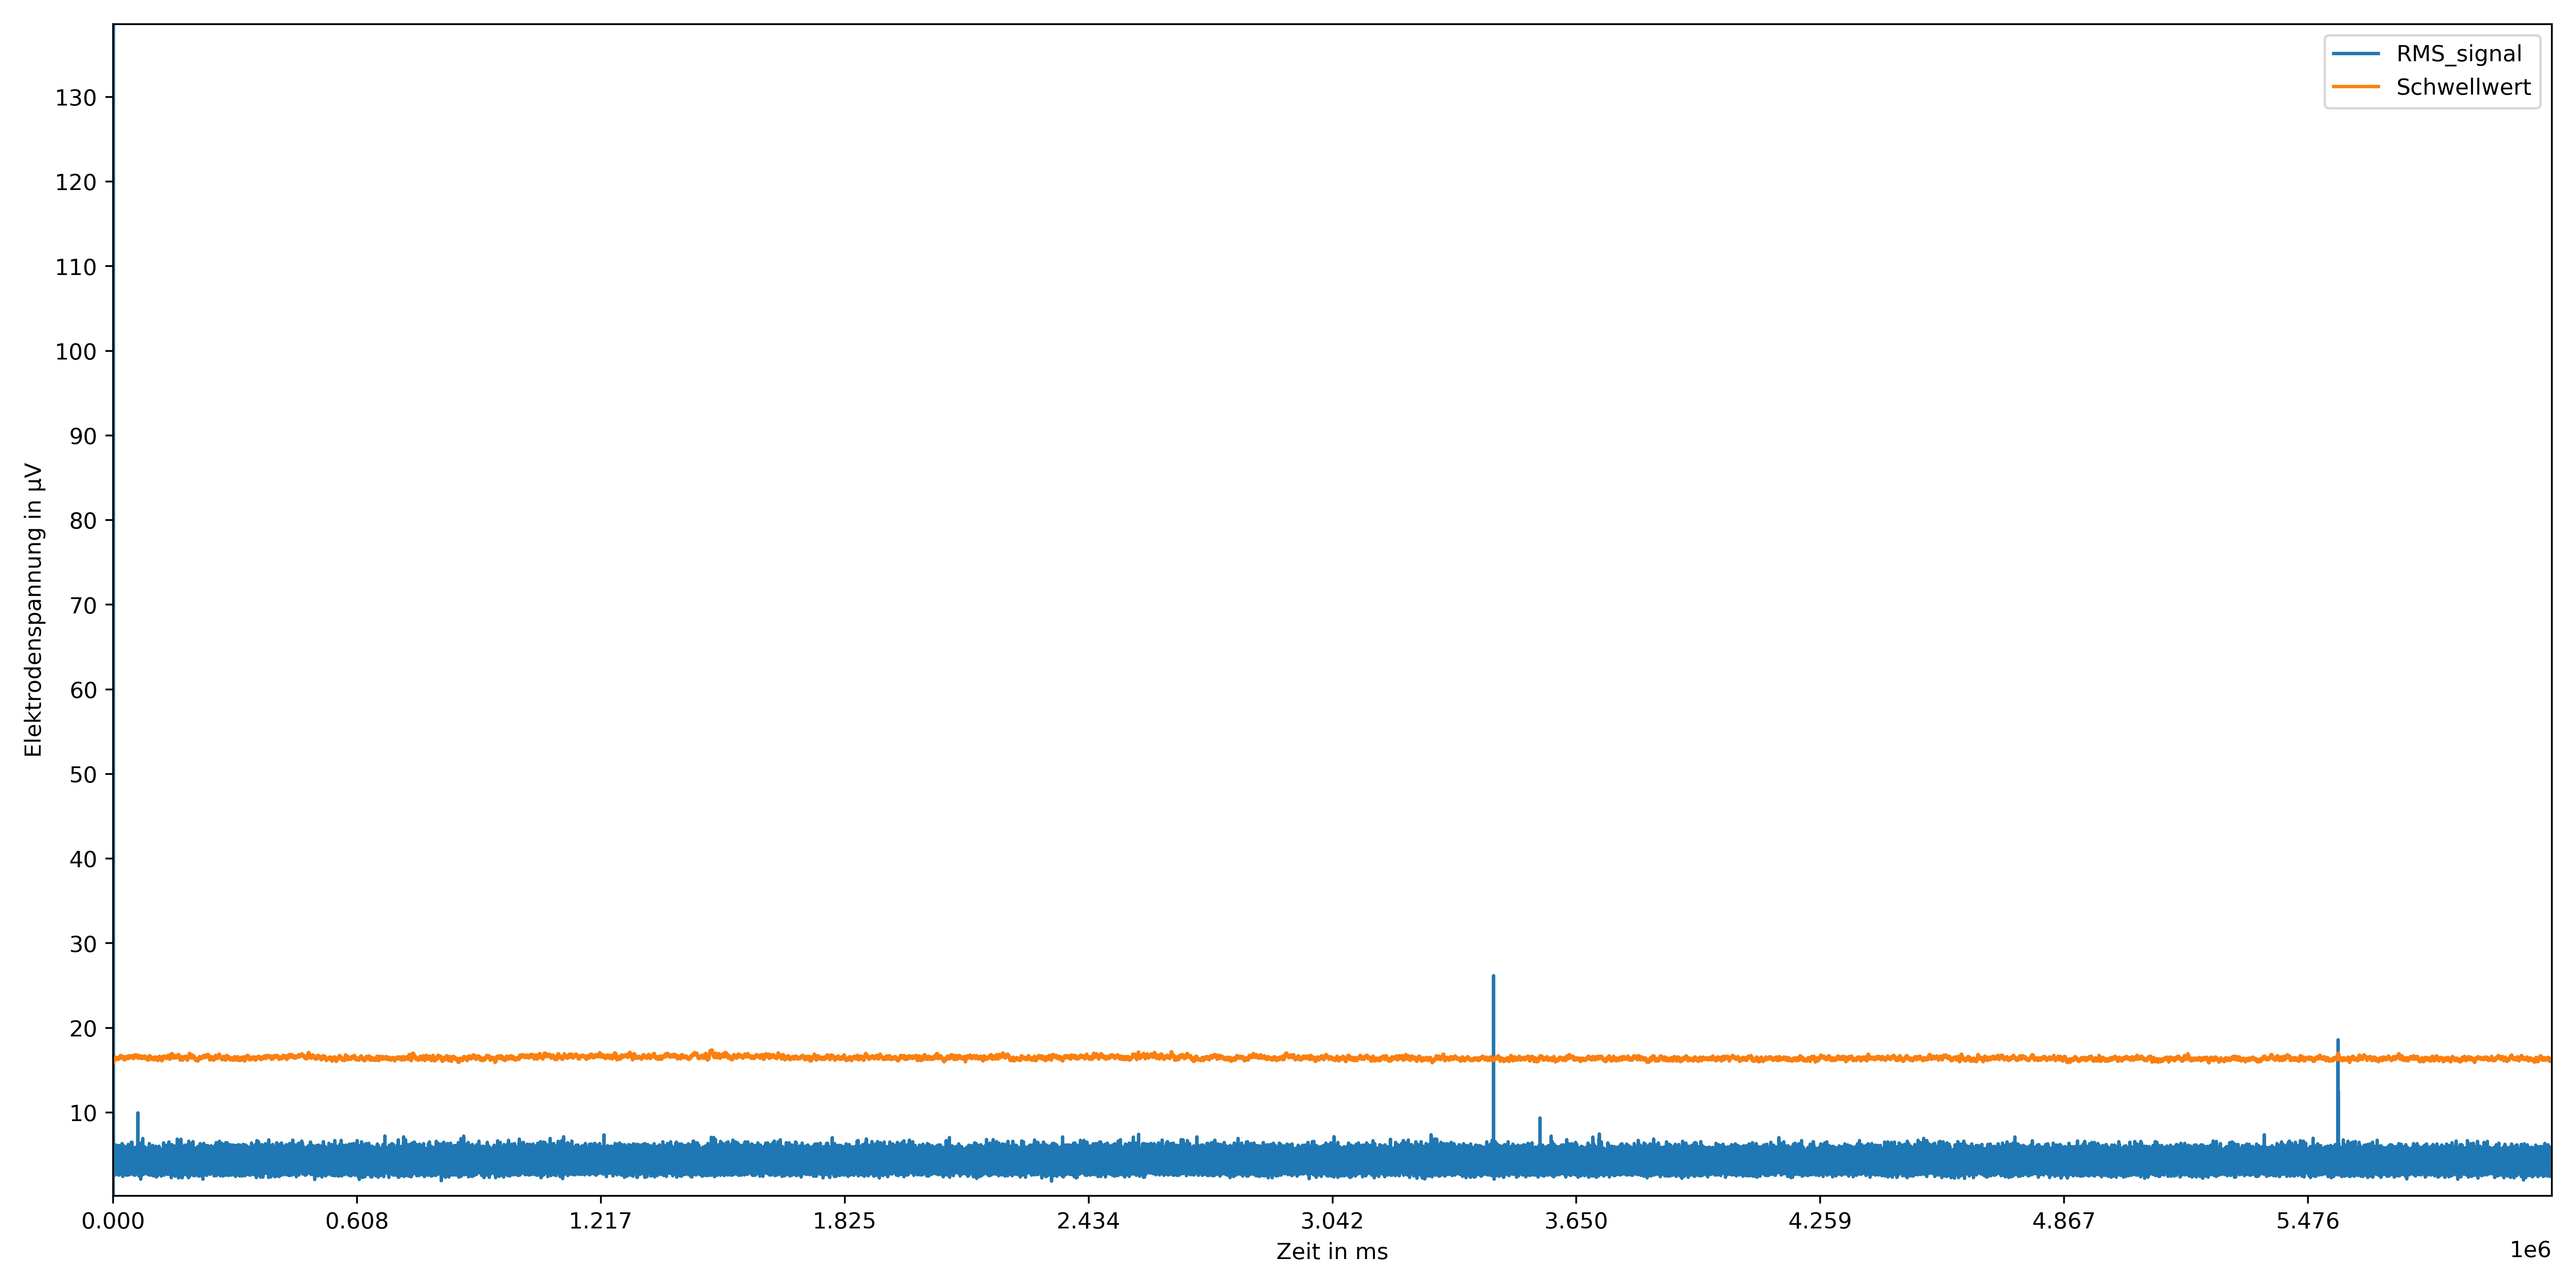
\includegraphics[width=0.80\textwidth]{./Bilder/flatSignalnohumanEMGacq_071085745.edf0,6084000.jpg}
	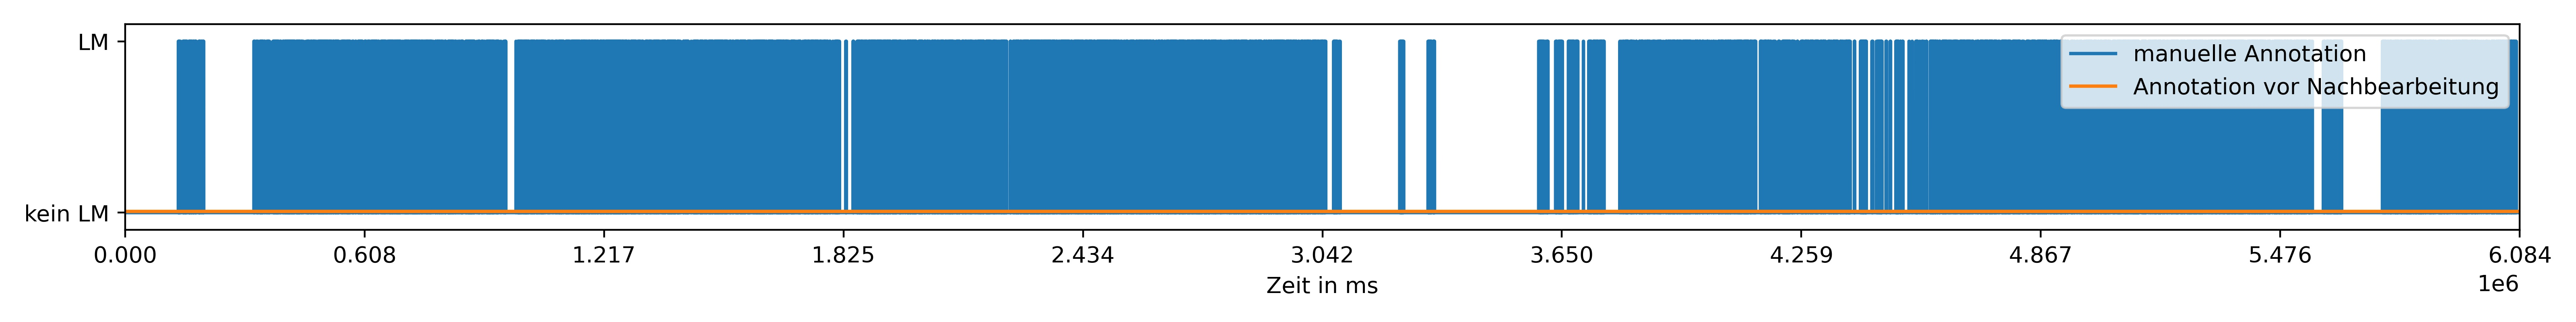
\includegraphics[width=0.80\textwidth]{./Bilder/flatSignalnohuman2acq_071085745.edf0,6084000.jpg}
	\end{center}
	\caption{Beispiel EMG-Signal mit Schwellwert (oben) und Annotationspaar (unten), bei der augenscheinlich keine Beinbewegungen stattgefunden haben. Die manuelle Annotation weist trotzdem viele Events auf.}%
	\label{fig:flat}%
\end{figure}



\begin{figure}[!ht]%
	\begin{center}
	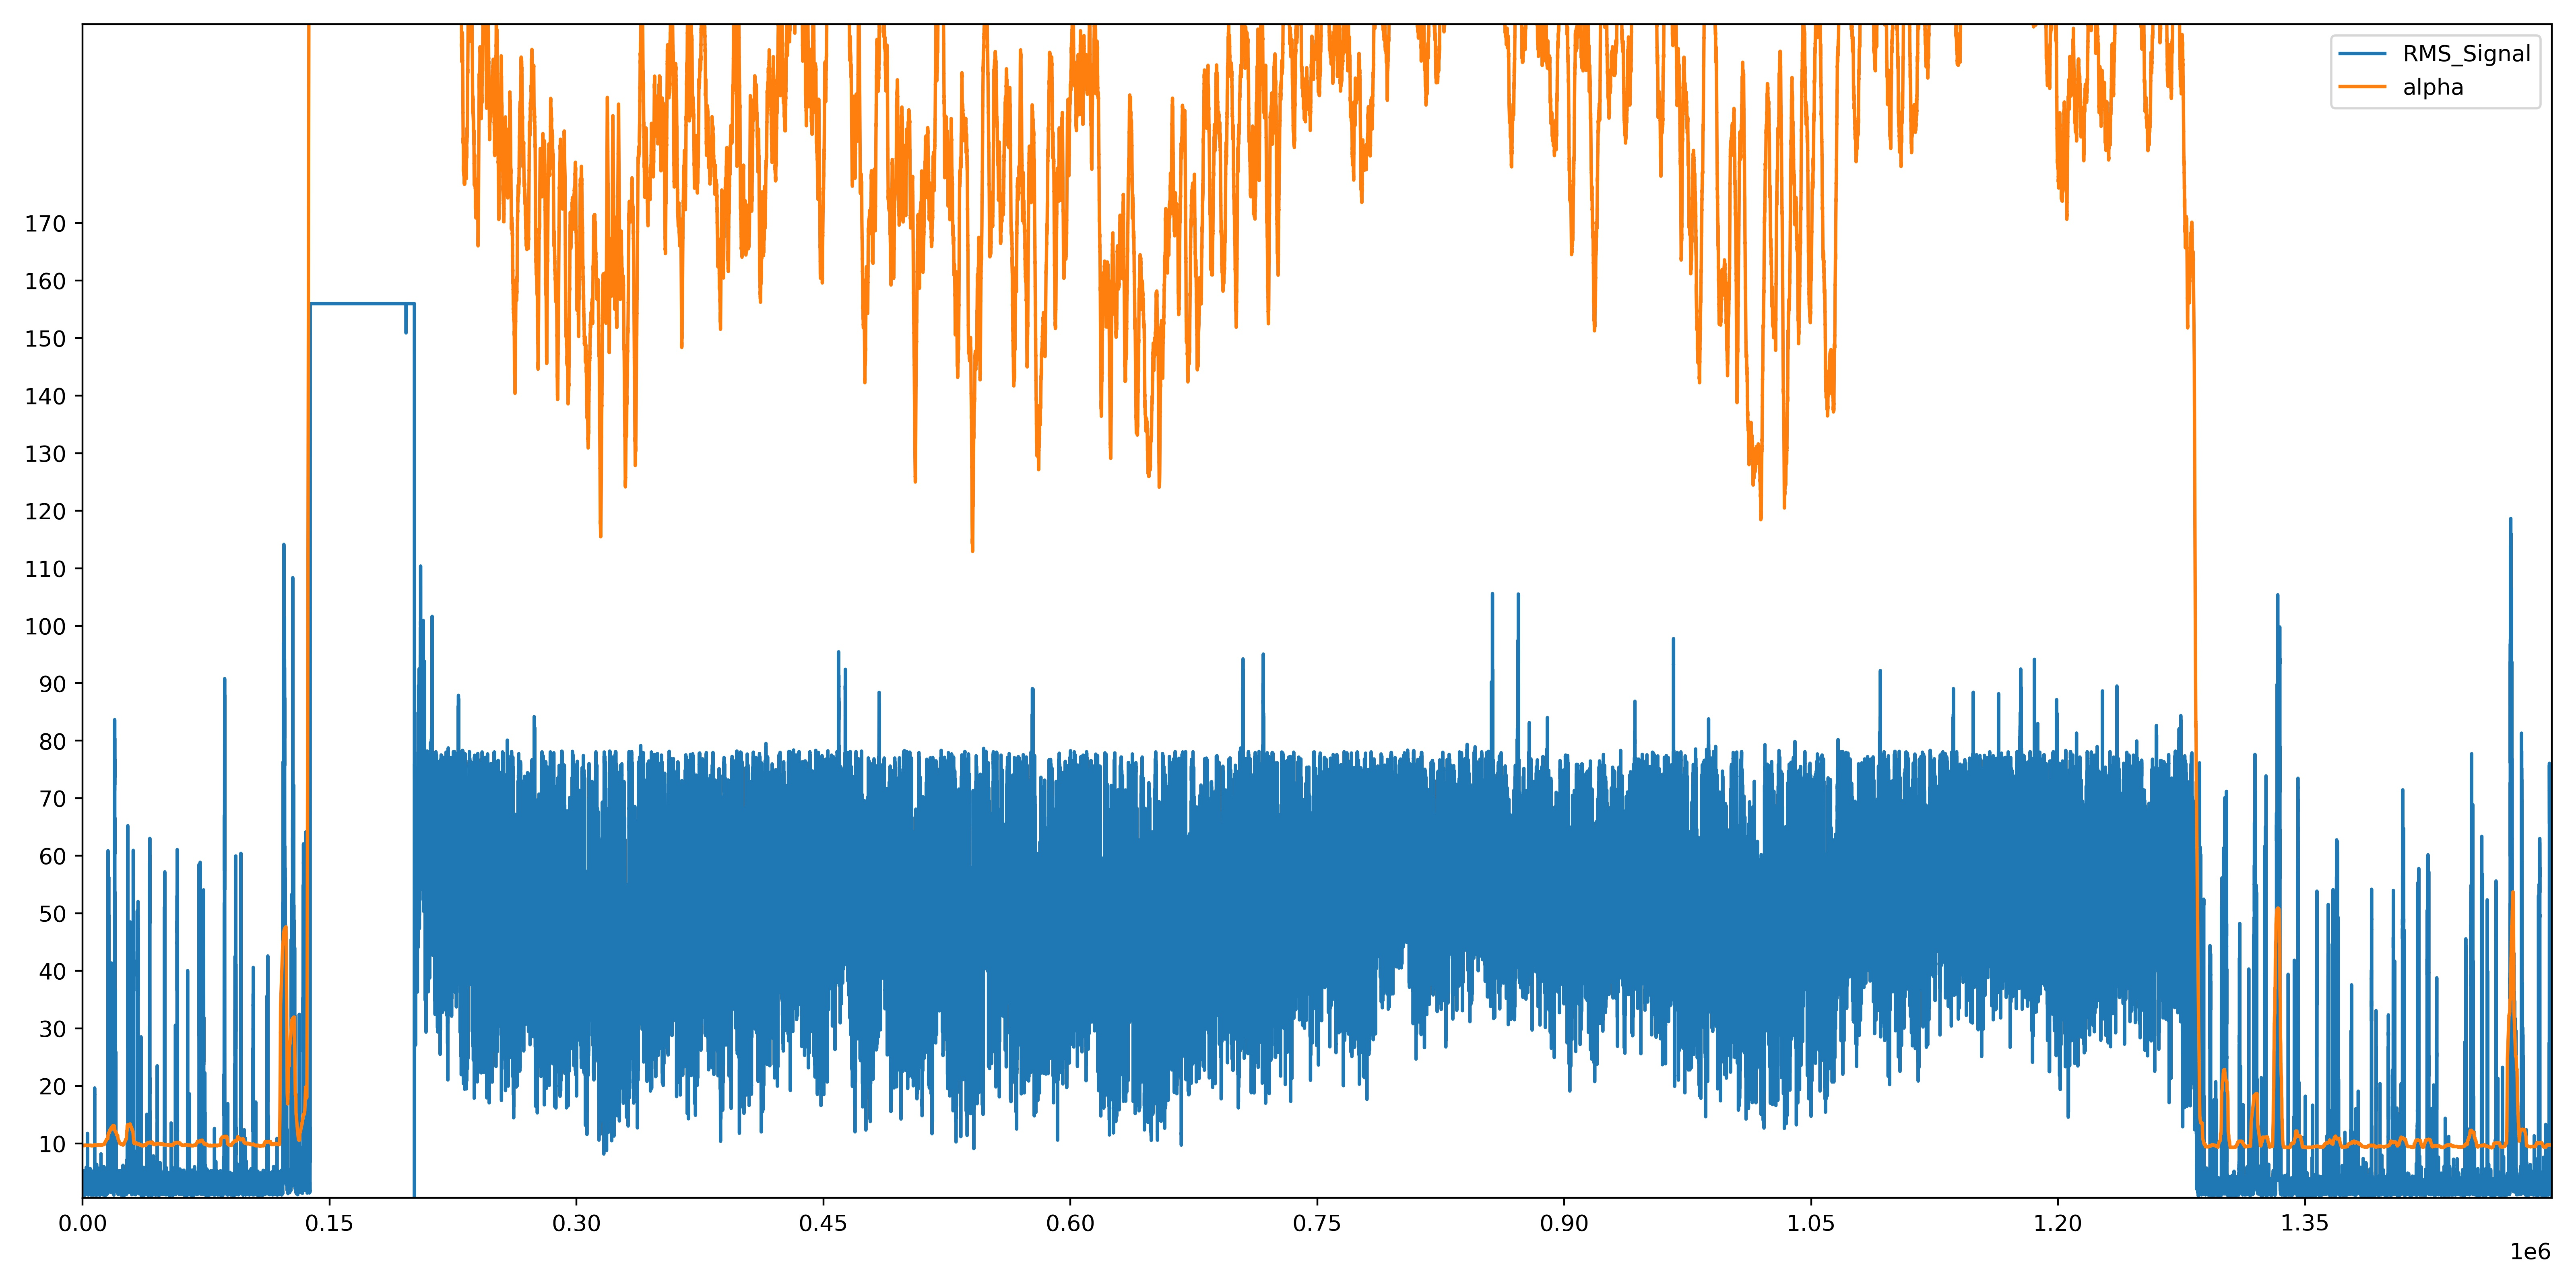
\includegraphics[width=0.80\textwidth]{./Bilder/badData1EMGacq_000952490.edf4000000,1500000.jpg}
	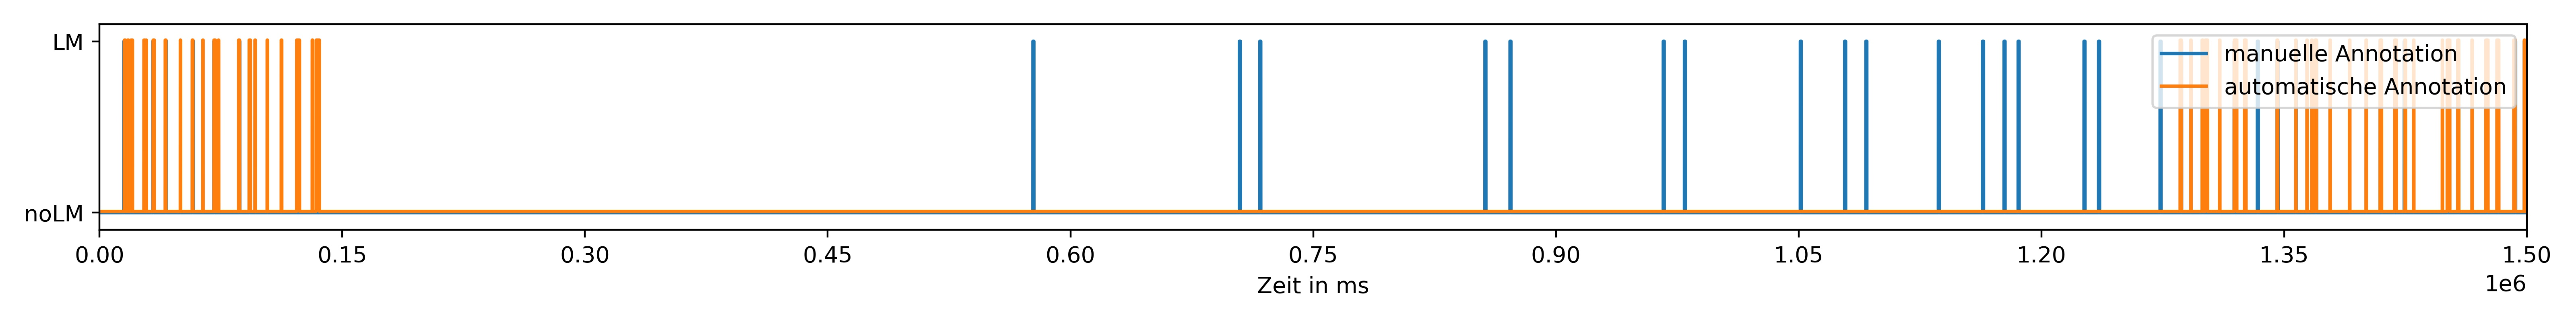
\includegraphics[width=0.80\textwidth]{./Bilder/badData1acq_000952490.edf4000000,1500000.jpg}
	\end{center}
	\caption{Ausschnitt eines EMG-Signals mit zeitweise schlechter Signalqualität (oben); laut manueller Annotation wurden in diesem Bereich trotzdem LMs gefunden (unten)}%
	\label{fig:Signalquali}%
\end{figure}

In der Abbildung \ref{fig:flat} ist ein EMG-Signal zu sehen, welches keine nenneswerten Ausschläge aufgezeichenet hat.
Die manuelle Annotation erkennt in diesem Signal sehr viele Events und es ist zu vermuten, dass das Signal von einer Annotationsunterstützung erstellt und nicht von Schlafspezialisten begutachtet wurde, bevor es in den Datensatz aufgenommen wurde.
Das Beispiel in Abbildung \ref{fig:Signalquali} zeigt eine zeitlich begrenzte Verschlechterung der Signalqualität, welche von dem dynamischen Schwellwert erkannt wird.
Zu beachten ist, dass die manuelle Annnotation in diesem Zeitraum Events aufweist.
Wahrscheinlich war nicht für alle Patienten eine explizite Untersuchung auf Beinbewegungen indiziert, sodass die Annotation möglicherweise nicht immer von Schlafspezialisten überprüft wurde. Die manuelle Annotation wurde vermutlich in diesen Fällen von einer Annotationsunterstützung erstellt.
Der Detektor wird in diesen Fällen auch an der manuellen Annotation bewertet und erzielt damit wesentlich schlechtere Ergebnisse. Die Grenzfälle mit einer sehr großen Abweichung zwischen manueller und automatischer Annotation beeinflussen den Mittelwert stark.
Die hier erzeugten Ergebnisse erlauben somit keinen Vergleich mit Detektoren, die auf anderen Datensätzen angewendet wurden.

Um die Qualtität des Datensatzes zu verbessern, empfiehlt die AASM für die Schwellwertklassifikation mit $8 \mu V$ und $2 \mu V$ Schwellwerten ein Ruhe-EMG-Signal dessen Amplitude kleiner als $\pm 10 \mu V_{pp}$. Da hier in dem gewählten Detektor ein dynamischer Schwellwert genutzt wird, kann für diese Arbeit nicht definiert werden ab welcher Grundrauschamplitude Signale ausgeschlossen werden können.


Selbst bei einem hochqualitativen Datensatz kann die manuelle Annotation von der Wirklichkeit abweichen. In der Veröffentlichung von Wetter et al. wird die Sensitivität zwischen zwei menschlichen Experten mit 97\% und die Präzision mit nur 92\% angegeben. Diese Abweichung ist für die Bewertung eines Detektors kritisch, da selbst ein hypothetisch perfekt funktionierender Detektor keine perfekten Ergebnisse hervorbringen würde. 
In Huang et al. wurde der Datensatz zusätzlich von Schlafexperten mit jahrelanger Erfahrung ausgewertet und hat somit zu einer besseren Bewertung des Detektors geführt (87.7\% im Vergleich zu 94.4\% Übereinstimmung). Bei Carvelli et al. wurde ein Konsens aus mehreren Schlafspezialisten durchgeführt um die Wirklichkeit zu approximieren. 
Diese Optionen waren für den gegebenen Datensatz nicht vorhanden. 
Da die Detektoren nur untereinander verglichen werden müssen reicht es aus die gleichen Ausgangsbedingungen für die Detektoren zu schaffen. Um die gleichen Bedingungen herzustellen sollten Detektoren nur vergleichen werden, wenn sie auf dem gleichen Datensatz getestet wurden.
Dies wird deutlich in dem Vergleich der Ergebnisse des Detektors von Moore et al., welcher auf den Daten von Alvarez-Estevez wesentlich schlechtere Ergebnisse liefert obwohl der gleiche Algorithmus verwendet wurde.


\section{Kostenfunktional}

Dass das Kostenfunktional nur sehr schwach mit den klassischen Metriken korreliert, ist damit zu begründen, dass die Ergebnisse des hier implementierten Detektors stark von den manuellen Annotationen abweichen. Dies ist insbesondere an dem kleinen Korrelationskoeffizienten der PLM-Indices zu erkennen.

Ein Problem bei der eventweisen Klassifikation ist, dass ein Abtastwert den Unterschied in der Anzahl der LM bedeuten kann. Da die Entscheidung welche der LM einander zugeordnet werden intuitiv von der Umgebung abhängt, ist es nicht einfach Regeln zu definieren, wann ein TP gezählt werden sollte.

Beim Bewerten des Detektors wurden Fehler ausschließlich anhand des binären Annotationssignals ohne vertiefende Fachkenntnis eines Schlafspezialisten definiert. Diese hätten möglicherweise bestimmte Fehler anders beurteilt, sodass sie in dem medizinischen Kontext ein aussagekräftigeres Ergebnis lieferten. 

Aufgrund der Definition der Güte \ref{Güte} der relativen Kosten kommt es außerdem zu einer Verzerrung der Interpretation bei gut funktionierenden Detektoren. Falls die relativen Kosten sehr klein sind und die Differenz der relativen Kosten zweier Detektoren relativ klein ist, wird es aufgrund der Nichtlinearität der Güte zu einem unerwartet großen Unterschied kommen. Die Güte ist also für kleine Kosten schlechter konditioniert. Das hat aber zusätzlich den Vorteil, dass sehr ähnliche Detektoren gut voneinander getrennt werden können.

Aufgrund dessen, dass für das Kostenfunktional Fehler gezählt werden, gibt es keine Obergrenze die der Wert annehmen kann. Die untere Grenze liegt bei Null. Das bedeutet auch, dass die Güte (zumindest bei unendlicher Signallänge) unendlich sein kann, wenn keine Fehler gemacht werden. 
Falls manuell keine PLM-Serien erkannt werden, sind die relativen Kosten wenig aussagekräftig, und gehen gegen unendlich, auch wenn nur ein Fehler gemacht wird. Wenn zusätzlich keine PLM-Serien vom Detektor erkannt werden, sind Kosten und Güte nicht definiert. Signale ohne manuelle Annotation sollten aus diesem Grund nicht zur Bewertung verwendet werden. 

Ein weiteres Problem ist, dass es bei einer PLM-Serie mehrere Gründe geben kann, warum diese fehlerhaft sind. So kann es beispielsweise dazu kommen, dass der erste TP eines 1toX-Matchings (welches die Serie verändert) gleichzeitig fälschlicherweise die [5-90] Sekunden Intervallgrenze überschreitet. 
Diese Fehler werden in der Aufschlüsselung der Kosten bei beiden Gründen sichtbar. Im Kostenfunktional wird in solchen Fällen nur ein Fehler gezählt.
Das Problem mit der Berechnung des Kostenfunktionals ist, dass es möglicherweise noch wesentlich mehr Grenzfälle gibt, als in dem in dieser Arbeit in Betracht gezogen wurden. Es eignet sich hierfür eine Implementierung, bei der für jedes LM die Gründe für die Fehler analysiert werden, anstatt für jeden Fehlergrund die LM zu suchen, die dagegen verstoßen.

Die Formel \ref{kdiff} $$
\overset{\text{ergebniserhöhende Fehler \textminus \ ergebnisverkleinernde Fehler}}{\underset{\text{automatisch annotierte PLM \textminus \ manuell annotierte PLM}}{=}}
$$
beschreibt inwieweit die Fehler, die von dem Detektor verursacht wurden, (PLM Differenz) von dem Kostenfunktional (Differenz aus Zuvielzählen und Zuwenigzählen) erklärt werden können. 
Da diese beiden Differenzen stark korreliert sind ($r^{2} = 0.99 $), kann geschlussfolgert werden, dass Kostenfunktional eine zuverlässige Beschreibung der Güte des Detektors ist.
Die weitere Untersuchung auf unbekannte Grenzfälle vernachlässigt werden, da diese das Ergebnis nur wenig beeinflussen.

Das Kostenfunktional ist auf die Kriterien der AASM zur Erkennung von PLM spezialisiert und kann deswegen auch nur in diesem Rahmen angewandt werden. Sollten sich diese Regeln ändern oder wird ein anderes Regelwerk bevorzugt, müssen die hier vorgeschlagenen Berechnungen angepasst werden und es lassen sich somit auch keine Vergleiche mehr zwischen den Bewertungen vor dieser Regeländerung herstellen. 
Die Prinzipien, für die Erstellung des Kostenfunktionals können auf ähnliche regelbasierte medizinische Fragestellungen angewandt werden. 


\section{Verbesserung der Einordnung des Detektors}
Da einige Gründe bekannt sind, aus denen die manuelle Annotation fehlerhaft sein könnte, bietet es sich an, die erhobenen Metriken aus dem Kapitel Verbesserung der Einordnung  des Detektors (Kapitel \ref{Verbesserung}) zu nutzen, um die Qualität des Datensatzes zu verbessern. 
Im Folgenden sind einige dieser Gründe aufgezählt und interpretiert.
Zuerst kann die Annahme getroffen werden, dass der Detektor seine Annotationsentscheidungen nur anhand der vorliegenden Daten trifft. Bei einer manuellen Annotation können andere Faktoren wie Monotoniemüdigkeit (siehe \ref{chap:Einleitung}) eine Rolle spielen. Sind beispielsweise Annotationspaare vorhanden, bei denen die manuelle Annotation ausschließlich im vorderen Teil der Nacht befinden, während automatische Annotationen über die ganze Nacht verteilt sind, könnte das bedeuten, dass die manuelle Annotation aus unbekannten Gründen abgebrochen wurde.

Die Teilmenge an Daten die vorzeitig abgebrochen wurde, weist tendenziell eine größere Abweichung der Schwerpunktdifferenz auf. Ein Extrembeispiel dafür könnte in Abbildung \ref{fig:noisy} zu sehen sein. Hier könnte die hohe Eventdichte für einen frühzeitigen Abbruch der manuellen Annotation geführt haben. Die Schwerpunktdifferenz liegt in dem folgenden Beispiel bei 3.03 Stunden.


\begin{figure}[!ht]%
	\begin{center}
	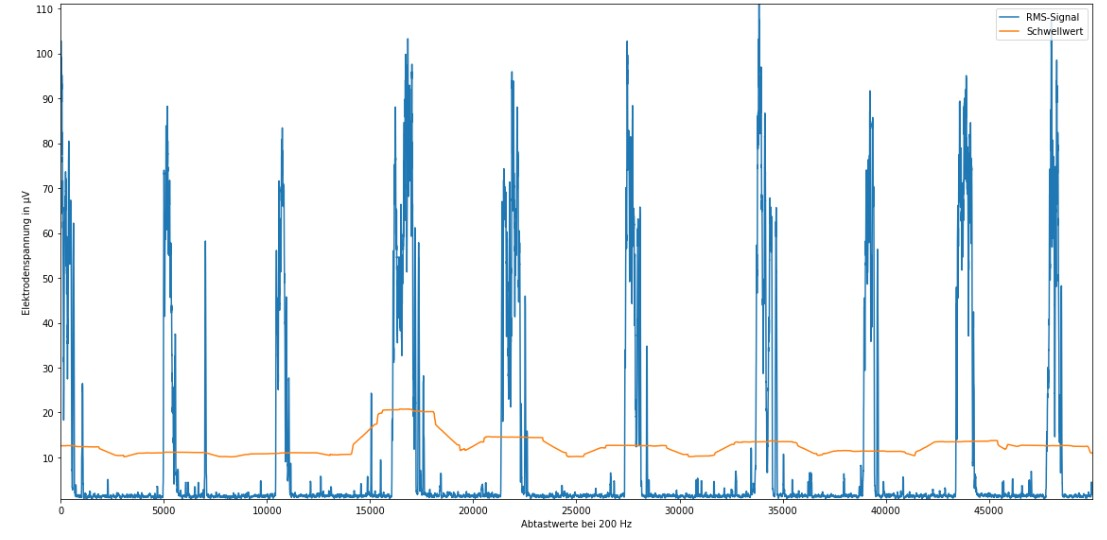
\includegraphics[width=0.80\textwidth]{./Bilder/starkesRauschenzoomedEMGacq_424517352.edf0,6516000.jpg}
	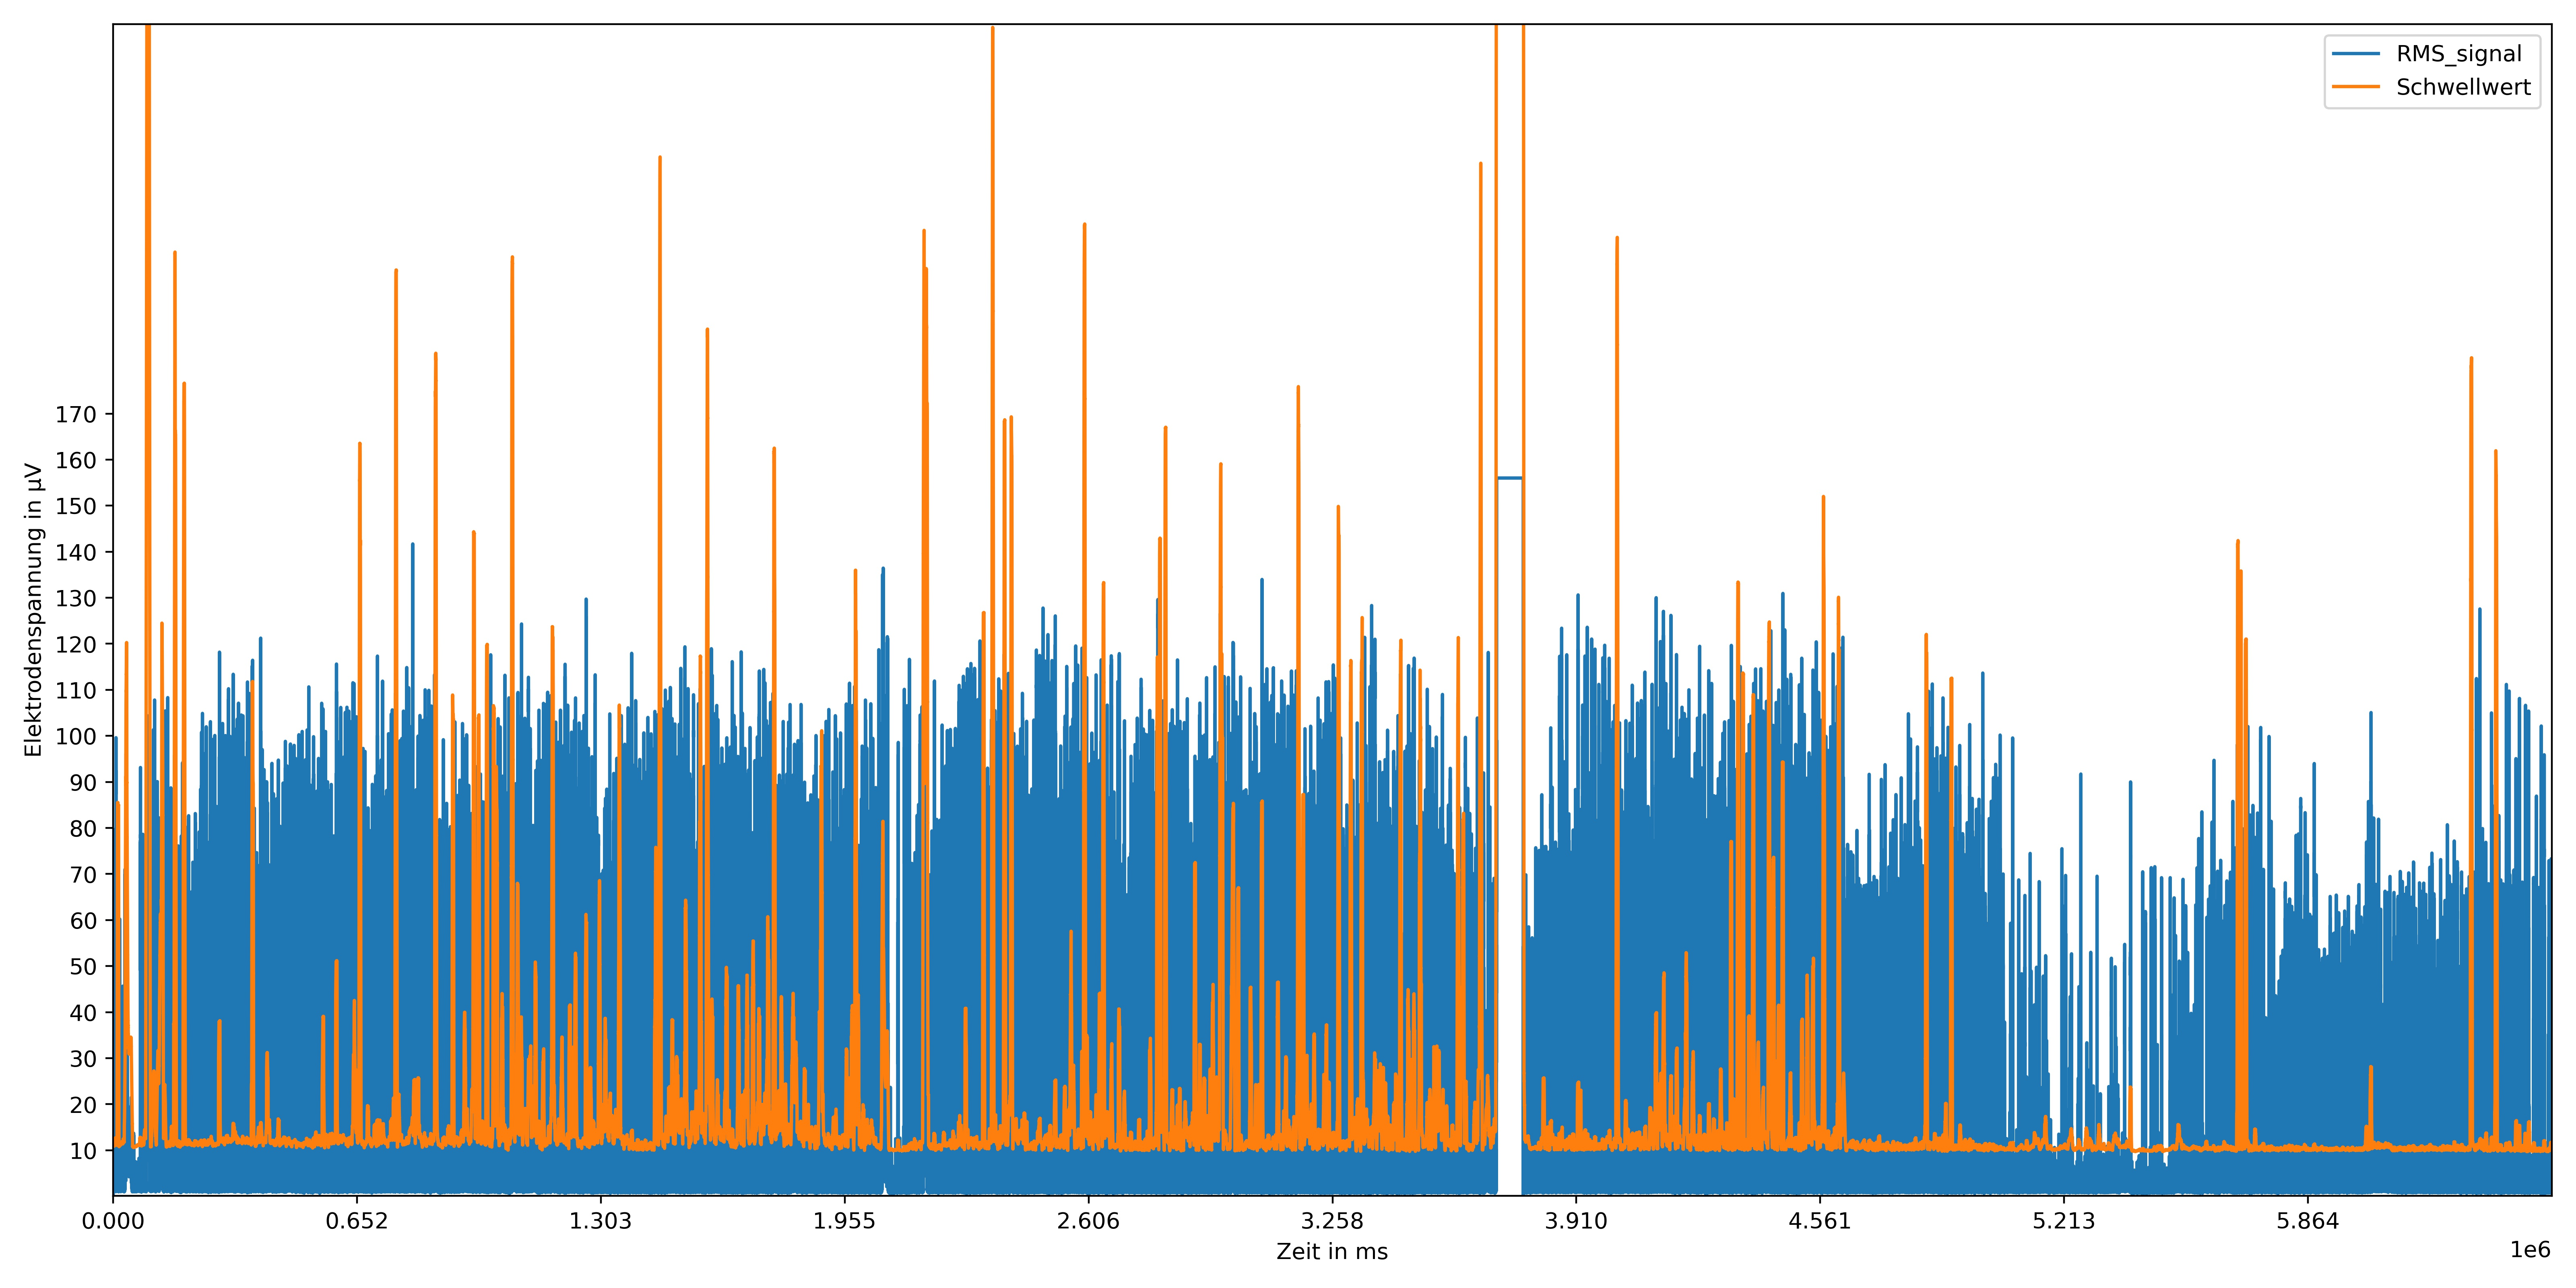
\includegraphics[width=0.80\textwidth]{./Bilder/starkesRauschenEMGacq_424517352.edf0,6516000.jpg}	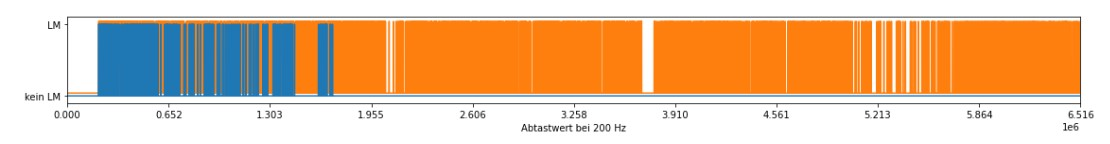
\includegraphics[width=0.80\textwidth]{./Bilder/starkesRauschen2acq_424517352.edf0,6516000.jpg}
	\end{center}
	\caption{Ausschnitt eines EMG-Signals mit sehr hoher Eventdichte(oben); das selbe EMG-Signal über die ganze Nacht dargestellt (mittig) mit zugehörigen Annotationen (unten); welche eine hohe Schwerpunktdifferenz aufweisen.}%
	\label{fig:noisy}%
\end{figure}


Im Histogramm \ref{fig:centers} ist eine solche Teilmenge weit entfernt von dem Mittelwert. Es kann jedoch ohne medizinisches Fachwissen kein Schwellwert definiert werden, unter dem die Daten aussortiert werden könnten. 


Bei einer segmentweisen manuellen Annotation wird der tatsächliche Startzeitpunkt in die Segmente diskretisiert. Da die meisten Detektoren quasizeitkontinuierlich auswertet, kann dieser bei ausreichend guter Detektionsqualität die Wirklichkeit zeitlich genauer darstellen. 
Gäbe es beispielsweise einen ungenau annotierenden Angestellten, der jede echte Beinbewegung eine Sekunde vorher (gerundet auf die Segmentgrenzen) schon als positiv markiert, würde der daraus resultierende Mittelwert der Startzeitpunkte über diese Nacht gesehen einen Ausreißer im Histogramm produzieren.
Diese Metrik könnte also einen Hinweis darauf geben, welche Dateien genauer untersucht werden sollten.
Es könnte argumentiert werden, dass Annotationen, welche im Mittel ungenauer sind als die Segmentgrenzen es zulassen, eher hinderlich für die Bewertung des Detektors sind, da die Startzeitpunkte den PLM-Index direkt beeinflussen.


Die Löschung von LM, die in der Nähe von atembezogenen Events stattgefunden haben, ist beispielsweise für den Detektor, ohne die benötigten Atem-Signale nicht zu erkennen. Unter der Annahme, dass diese Art von Events nicht bei allen Patienten auftritt, könnte es sinnvoll sein, die Nächte genauer zu untersuchen, bei der die falsch positiv Rate stark von dem Mittelwert abweicht. Anhand des  Histogramms \ref{fig:FPrate} aus den Ergebnissen, ist nicht zu erkennen, ab welchem Wert eine starke Abweichung zu vermuten ist. Diese Abweichung wird vermutlich erst bei sehr guten Ergebnissen sichtbar.


Ein sehr hohes LM Verhältnis bedeutet, dass der Detektor wesentlich öfter auf einen Anstieg im EMG-Signal reagiert als das medizinische Personal es tun würde. Diese Metrik könnte also einen Hinweis darauf geben, wie sinnvoll es ist, den Erkennungsschwellwert anzuheben. Die Aussage des Mittelwertes und des Medians ist für den implementierten Detektor widersprüchlich. Betrachtet man das die Differenz der gefundenen LM (automatisch gefundene LM – manuell gefundene LM) wird ersichtlich, dass der Detektor in den meisten Fällen weniger LM als das medizinische Personal erkennt. Im Durchschnitt erkennt der Detektor 87.1 von 226 Beinbewegungen zu wenig. In diesem Fall könnte also die Formel für den Schwellwert angepasst werden, sodass mehr LM erkannt werden. 



Eine hohe Anzahl an 1toX-Matches impliziert, dass der Detektor das Ende eines LM zu früh erkennt. In diesen Fällen könnte beispielsweise eine Änderung in den Zeiten der Nachbearbeitung des Annotationssignals oder die Definition des unteren Schwellwertes angepasst werden. Die Anzahl der Xto1-Matches trifft entgegengesetzte Aussagen. In dem hier implementierten Detektor sind beide Anzahlen nicht besonders hoch.
Falls es Verstöße gegen die definierte Länge der LM gibt, könnte das bedeuten, dass der Detektor entweder Ausschläge im EMG als LM klassifiziert, die nicht aus Beinbewegungen stammen oder die Dauer eines richtig gefundenen LM wird falsch eingeschätzt. Diese Metrik ist für den Detektor per Definition bei Null, da in der Nachbearbeitung des Annotationssignals die Länge der gefundenen LM überprüft wird.


Die Mittelwerte der Verteilung (über alle Nächte berechnet) kann genutzt werden, um den Detektor auf systematische Fehler zu untersuchen. Liegen beide Mittelwerte bezogen auf die manuelle Annotation zeitlich gesehen im positiven Bereich, kann das darauf hindeuten, dass die Vorverarbeitung des EMG-Signals einen zu starken Tiefpasscharakter aufweist und somit die Flanken der LM weniger schnell ansteigen und abfallen. Dies würde dazu führen, dass alle automatisch erkannten LM leicht zeitlich versetzt zu den korrespondierenden manuell erkannten LM sind.
Es ist zu vermuten, dass in der manuellen Annotation auch systematische Fehler gemacht wurden. Da die Mittelwerte der Startzeitpunkte negativ und die Mittelwerte der Endzeitpunkte positiv sind, lässt sich vermuten, dass das medizinische Personal, anstatt exakt ab- und aufzurunden, lieber das ganze Segment als positiv definiert hat, in dem ein LM stattgefunden hat.
Aus diesem Grund können systematische Fehler nur zwischen den Detektoren untereinander verglichen werden.

Maschinelle Lernalgorithmen sind aufgrund der hohen Anzahl der Parameter in der Lage sich an den Trainingsdatensatz stark anzupassen. Es kann also passieren, dass der Algorithmus die Segmentierung der Annotation mitlernt, obwohl diese in dem Eingangssignal nicht vorhanden sind.
Die Verteilung der LM-Startzeitpunkte hat aufgrund der Segmentierung der manuellen Annotation eine bestimmte Standardabweichung. Wird von einem Detektor, der mithilfe eines solchen Lernalgorithmusses arbeitet diese Standardabweichung unterschritten, könnte eine Überanpassung an die Segmentgrenzen stattgefunden haben. Diese Überanpassung lässt sich anhand dieser Metrik feststellen. 
Ein Neuronales Netz welches die Segmentgrenzen auswendig gelernt hat, würde auf einem anderen Datensatz mit quasikontinulierlicher manueller Annotation eine unerwartet hohe Standardabweichung aufweisen und damit auch zu schlechteren Ergebnissen führen. Die Struktur eines Schwellwertdetektor hat zu wenig wählbare Parameter um Segmentgrenzen zu erlernen. Daher kann die Metrik hier nicht ausgewertet werden.



\section{Optimierung des Detektors}

Es sollte darauf geachtet werden, dass die Bewertung des Detektors nicht mit der Optimierung des Detektors vermischt wird. Da die Optimierung anhand der Metriken im Kapitel Verbesserung der Einordnung des Detektors (Kap. \ref{Verbesserung}) unabhängig von dem Kostenfunktional ist, können diese genutzt werden. 
Es wird trotzdem empfohlen die Bewertung des Detektors anhand von Daten durchzuführen, die nicht zu einer Veränderung des Detektors geführt haben.
Das Kostenfunktional lässt sich durch die Zählweise nicht mathematisch ableiten und kann somit nicht durch Optimierungsverfahren genutzt werden, die auf Gradienten beruhen. Trotzdem lassen sich Detektoren aufgrund der Definition einer Güte, welche als Inverse der Kosten definiert ist, durch Verfahren wie genetischen Algorithmen verbessern.